\documentclass{beamer}
\usepackage[ngerman]{babel}
\usepackage[utf8]{inputenc}
\usepackage{listings}
\usepackage{verbatim}
\usepackage{wrapfig}
\newcommand{\comments}[1]{}
\bibliographystyle{plain}

\setlength{\leftmargini}{10pt}

\usetheme{Berlin}
\usecolortheme{default}
\setbeamertemplate{navigation symbols}{}


\title[SMS Versendung über Datenkanäle]{SMS Versendung über Datenkanäle}
\author{Sebastian Menski \and Martin Ohmann}
\institute{Institut für Informatik -- Universität Potsdam}
\date{30. Juli 2012}
\begin{document}

\begin{frame}
\titlepage
\end{frame}


\begin{frame}{Inhalt}
\tableofcontents
\end{frame}

\section{SMS über GSM/GPRS} %{{{

\subsection{Entstehung}
\begin{frame}{Entstehung}
	\begin{itemize}
		\item Erste Überlegungen zu Textnachrichtendienst 1984 bei den 
			europäischen Telekommunikationsgesellschaften
		\item Verabschiedung der ersten Version des endgültigen Standards 
			Anfang 1989
		\item Erste SMS wurde am 3. Dezember 1992 von einem PC an ein 
			Mobiltelefon gesendet
	\end{itemize}
\end{frame}

\subsection{Technische Realisierung}
\begin{frame}{SMS-Spezifikationen}
	\begin{itemize}
		\item Maximale Payload beträgt 140 Bytes; Gewöhnlich 160 Zeichen mit 
			7-Bit-Encoding
		\item Segmentierung überlanger Nachrichten in mehrere Einzelnachrichten
		\item Versendung erfolgt über den GSM-Signalisierungskanal (SDCCH oder FACCH)
		\item Verwaltung gesendeter Nachrichten durch Short Message Service 
			Center (SMSC) des Providers
		\item SMSC arbeitet gewöhnlich nach Store-and-forward Prinzip
	\end{itemize}
\end{frame}

\begin{frame}{SMS-Aufbau}
	\begin{itemize}
		\item Header: enthält grundlegende Nachrichtenparameter wie z.B. 
			Empfängernummer, Nummer des SMSCs, Nachrichtenkodierung
		\item Body: enthält die Payload (max. 140 Bytes)
	\end{itemize}
	\begin{figure}[htm]
		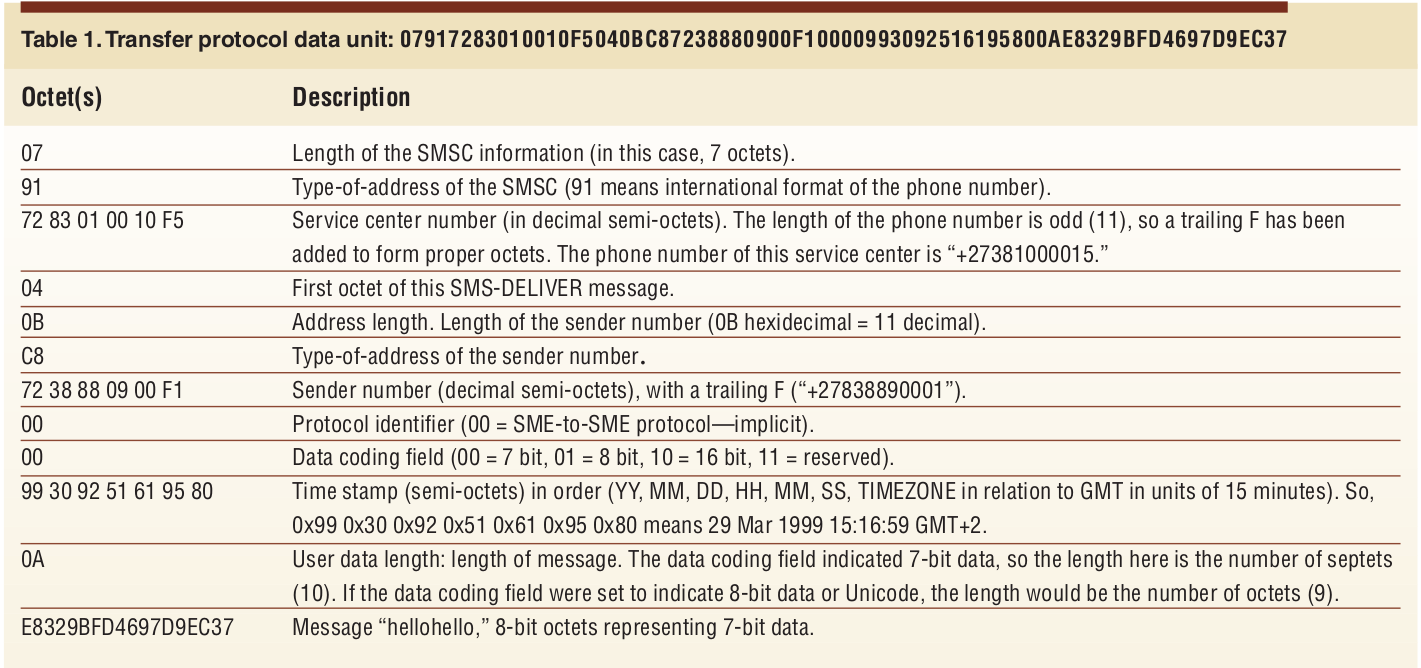
\includegraphics[width=0.9\textwidth]{img/tpdu-example.png}
		\label{tpdu-example}
	\end{figure}
\end{frame}

\begin{frame}{SMS-Versand}
	\begin{itemize}
		\item Realisiert durch den Mobile Application Part (MAP) des SS\#7 
			(Signaling System No. 7) Protokolls 
		\item Elemente des Short Message Protokolls werden als Felder innerhalb 
			von MAP Nachrichten durch das Netzwerk transportiert
		\item Vier MAP Prozeduren zur Kontrolle des Short Message Services:
			\begin{itemize}
				\item Mobile Originated (MO) short message service transfer
				\item Mobile Terminated (MT) short message service transfer
				\item Short message alert procedure
				\item Short message waiting data set procedure
			\end{itemize}
	\end{itemize}
\end{frame}

\begin{frame}{SMS-Versand -- Mobile Originated}

	\begin{itemize}
		\item Nachricht wird vom mobilen Endgerät über Funk zum Mobile Switching 
			Center/GRPS Core Network (VMSC/SGSN) geschickt
		\item VMSC/SGSN sendet mo-ForwardSM Operation an das zuständige SMSC 
			des Providers (Übermittlung von SMS-PP Application Protocol Data Unit (APDU))
		\item SMSC speichert Nachricht und versucht anschließend diese an die 
			Zieladresse auszuliefern
	\end{itemize}
\end{frame}

\begin{frame}{SMS-Versand -- Mobile Originated (2)}

	\begin{figure}[htm]
		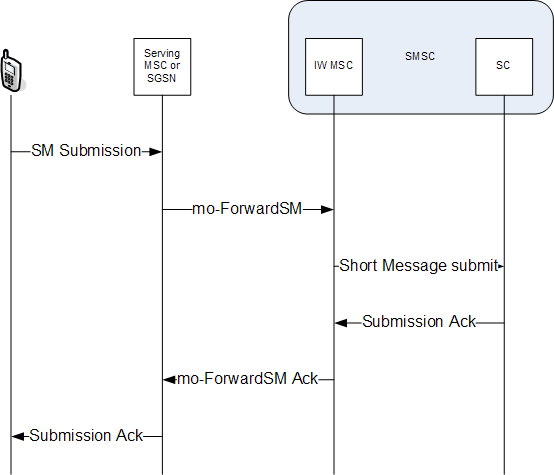
\includegraphics[width=0.65\textwidth]{img/mo-forward-sm.png}
		\label{mo-forward-sm}
	\end{figure}
\end{frame}

\begin{frame}{SMS-Versand -- Mobile Terminated}

	\begin{itemize}
		\item SMSC sendet SMS-PP APDU der Nachricht an die Gateway MSC (GMSC) 
			Komponente des SMSC
		\item GMSC fragt beim Home Location Register (HLR) Position des 
			Empfängers an (SRI-for-SM)
		\item GMSC sendet mt-ForwardSM Nachricht an die vom HLR bereitgestellte 
			Adresse des VMSC/SGSN
		\item Das VMSC/SGSN fragt die benötigten Informationen zum Ausliefern der Nachricht beim VLR 
			durch eine Send\_Info\_for\_MS\_SMS Nachricht ab
		\item Das VLR sucht nach dem 
			Empfänger und liefert die Mobile Subscriber ISDN Number (MSISDN) des Empfängers an 
			das VMSC zurück
	\end{itemize}
\end{frame}

\begin{frame}{SMS-Versand -- Mobile Terminated (2)}

	\begin{figure}[htm]
		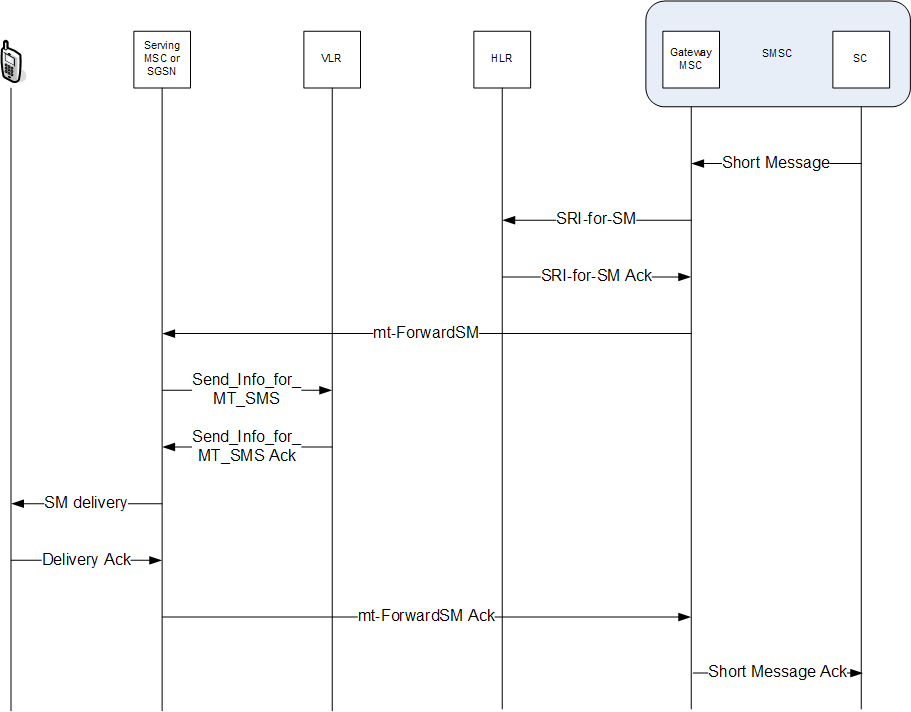
\includegraphics[width=0.7\textwidth]{img/mt-forward-sm.png}
		\label{mt-forward-sm}
	\end{figure}
\end{frame}

\subsection{Grenzen von SMS über GSM/GPRS}
\begin{frame}{Grenzen von SMS über GSM/GPRS}
	\begin{itemize}
		\item \textbf{Nicht Multi-Device tauglich}: SMS Service ist an eine einzige 
			Mobilfunknummer gebunden
		\item Kosten: SMS im Vergleich zu Kommunikation über Datennetz sehr 
			\textbf{teuer}
		\item \textbf{Keine Real-Time-Kommunikation} möglich; keine garantierten Zustellzeiten; 
			kein ``is typing''-Feature
		\item \textbf{Keine Gruppennachrichten} möglich
		\item Durch Limitation auf 160 7-Bit-Zeichen \textbf{keine Rich-Text-Nachrichten} 
			möglich
		\item Übertragungskanal ursprünglich nicht für das heutige 
			Nachrichtenaufkommen ausgelegt
	\end{itemize}
\end{frame}

% sms }}}

\section{SMS über Datennetze}
\begin{frame}{Datennetzbasierte SMS Alternativen}
	\begin{itemize}
		\item Viele Alternativen zur herkömmlichen SMS
	\end{itemize}
	\begin{figure}[htm]
		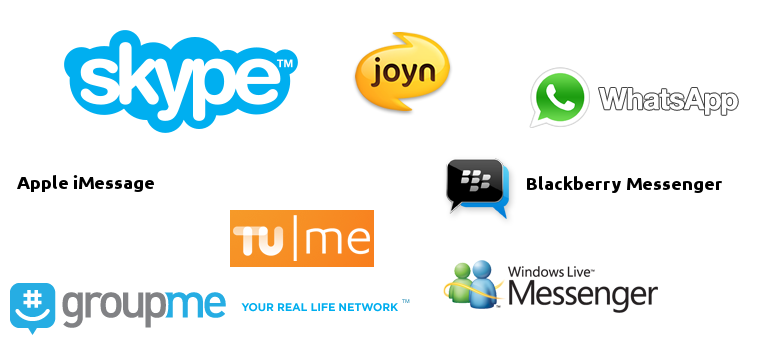
\includegraphics[width=\textwidth]{img/messengers.png}
		\label{messengers}
	\end{figure}
\end{frame}

\subsection{Hersteller-Service}
\begin{frame}{Hersteller-Service}
	\begin{itemize}
		\item Hersteller spezifischer Service
		\item Beispiele: iMessages (Apple), Blackberry Messenger
		\item Kunden können \textbf{untereinander} kostenlos über Nachrichten kommunizieren
		\item Keine Anmeldung nötig
		\item Ähnlich Instant Messaging
	\end{itemize}
\end{frame}

\subsection{Apps}
\begin{frame}{Apps}
	\begin{itemize}
		\item Apps für Smartphones von Drittanbietern
		\item Meist für alle wichtigen Platformen verfügbar
		\item Beispiele: WhatsApp, kik
		\item Kunden müssen sich anmelden oder werden über die Mobilfunknummer identifiziert
		\item Kostenlos oder geringe Kosten
		\item Ähnlich Instant Messaging
	\end{itemize}
\end{frame}

\subsection{RCS-e}
\begin{frame}{Rich Communication Suite-enhanced (RCS-e)}{Übersicht}
	\begin{itemize}
		\item Industriestandard für Kommunikation von mobilen Endgeräten
		\item Nutzt Standards von \textit{3GPP}, \textit{OMA} und \textit{IETF}
		\item Bestandteile:
		\begin{itemize}
			\item Präsenzinformation
			\item Sprachtelefonie
			\item Videoübertragung
			\item Datenaustausch
			\item Instant Messaging
			\item Ortung
		\end{itemize}
	\end{itemize}
\end{frame}

\begin{frame}{Rich Communication Suite-enhanced (RCS-e)}{Übersicht (2)\cite{rcs:spec}}
	\begin{figure}[htm]
		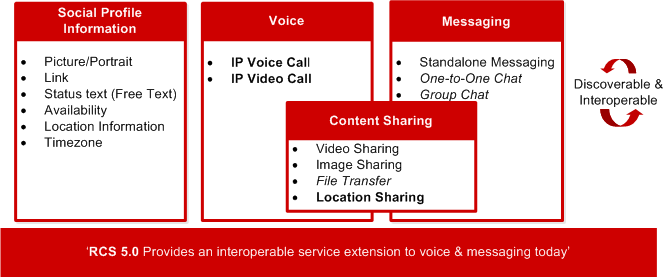
\includegraphics[width=0.65\textwidth]{img/rcs-e-overview}
	\end{figure}
\end{frame}

\begin{frame}{Rich Communication Suite-enhanced (RCS-e)}{Entwicklung}
	\begin{itemize}
		\item Entwicklungsstart: 2008
		\item Druch Branchenverband \textit{GSM Association (GSMA)} vorangetrieben
		\item Vermarktung unter dem Namen \textit{joyn} (\glqq{}Nachfolger der SMS\grqq{})
		\item Angekündigte Unterstützung der Betriebssysteme Windows Mobile, iOS und Android
		\item Anfangs durch Apps; Später integration ins OS
		\item Offizielle Premiere auf der \textit{GSMA Mobile World Congress 2012 (MWC)}
		\item Gleichzeitig Freigabe der Version 5.0 des Standards
	\end{itemize}
\end{frame}

\begin{frame}{Rich Communication Suite-enhanced (RCS-e)}{Einführung}
\begin{itemize}
	\item Vodafone Spanien startete Anfang 2012 eine Beta-Phase mit Android-App
	\item Vodafone Deutschland: \glqq{}angeblich\grqq{} im Juni 2012
	\item T-Mobile: Oktober 2012
	\item O2: 2013
\end{itemize}
\end{frame}


\begin{frame}{Rich Communication Suite-enhanced (RCS-e)}{Technik\cite{rcs:spec}}
	\begin{itemize}
		\item \textit{3GPP IP Multimedia Subsystem (IMS)} mit \textit{IETF Session Initiation Protocol (SIP)} zur:
			\begin{itemize}
				\item Authentifizierung
				\item Autorisierung
				\item Registrierung
				\item Abrechnung
			\end{itemize}
		\item \textit{Open Mobile Alliance (OMA)} Standards zur Kommunikation
		\item \textit{Standalone Messaging} ist die Weiterentwicklung der SMS/MMS
	\end{itemize}
\end{frame}

\begin{frame}{Rich Communication Suite-enhanced (RCS-e)}{Standalone Messaging\cite{rcs:spec}}
	Standalone Messaging:
	\begin{itemize}
		\item Text- und Multimedia-Nachrichten
		\item Versand- und Displaymitteilungen
		\item Multi-Device Unterstützung
		\item Zentraler und lokaler Nachrichtenspeicher
		\item Unterstützung alten Nachrichtensysteme (SMS, MMS)
		\item nutzt \textit{OMA Converged IP Messaging (CPM)} im Pager und Large Message Mode
		\item Pager Mode: Begrenzung auf 1300 Byte
	\end{itemize}
\end{frame}

\begin{frame}{Rich Communication Suite-enhanced (RCS-e)}{CPM Pager Mode\cite{rcs:spec}}
	\begin{figure}[htm]
		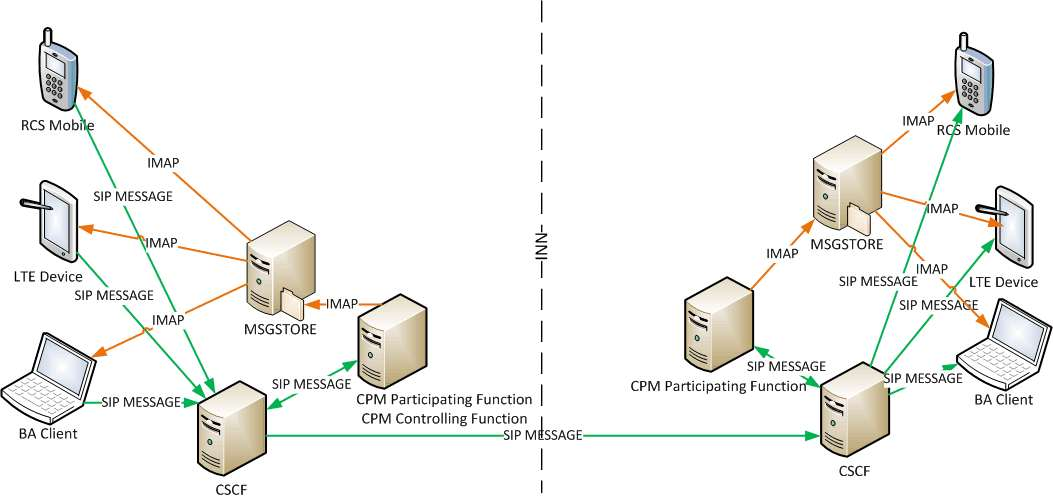
\includegraphics[width=0.85\textwidth]{img/rcs-e-pager}
	\end{figure}
\end{frame}

\begin{frame}{Rich Communication Suite-enhanced (RCS-e)}{CPM Large Mode\cite{rcs:spec}}
	\begin{figure}[htm]
		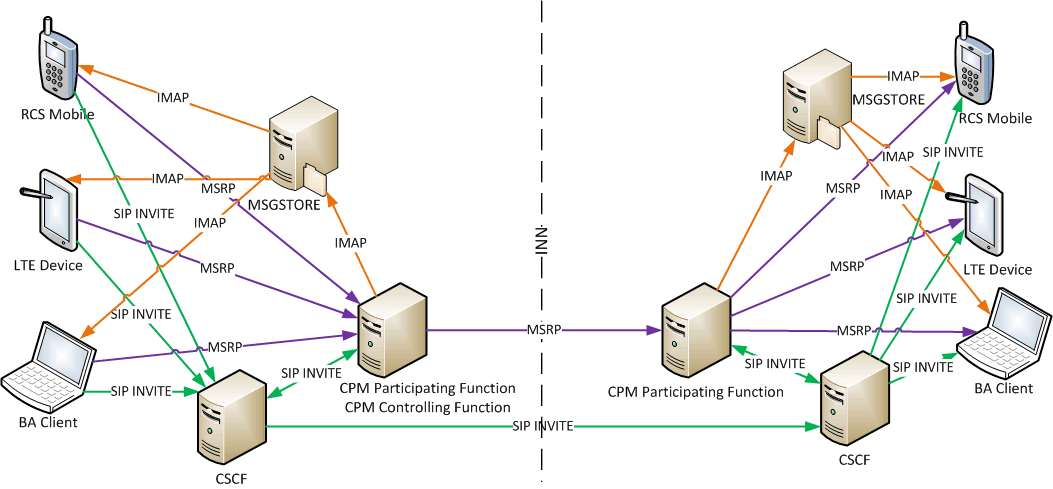
\includegraphics[width=0.85\textwidth]{img/rcs-e-large}
	\end{figure}
\end{frame}

\begin{frame}{Rich Communication Suite-enhanced (RCS-e)}{SMS Unterstützung\cite{rcs:spec}}
	\begin{figure}[htm]
		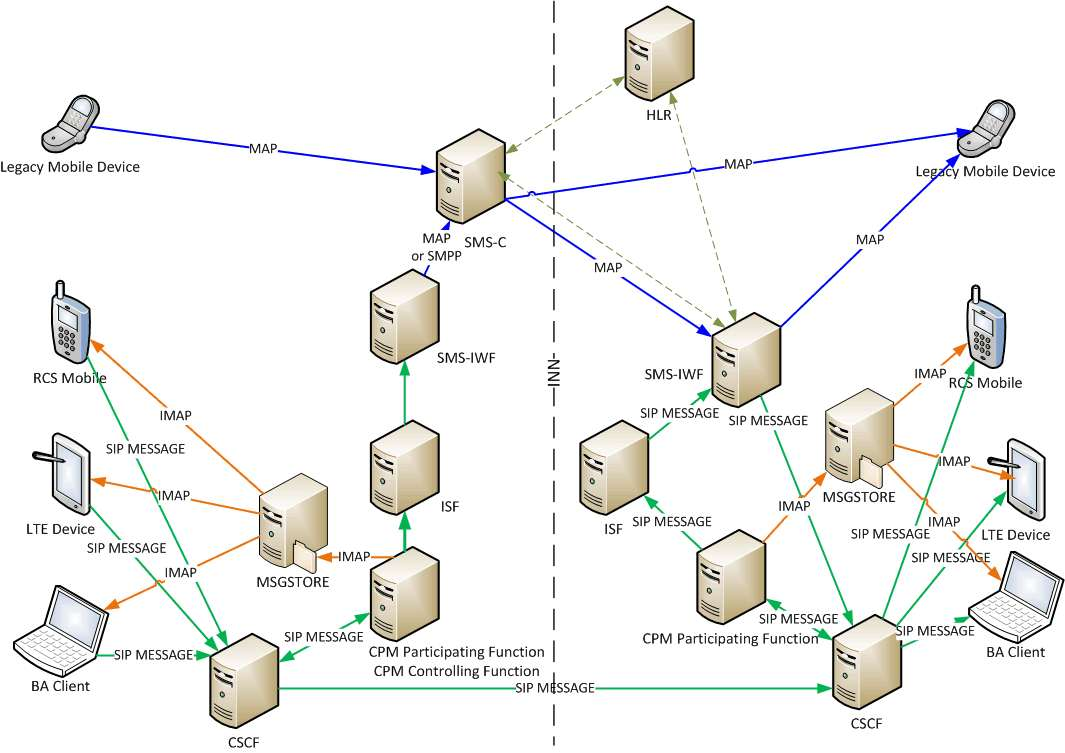
\includegraphics[width=0.75\textwidth]{img/rcs-e-sms}
	\end{figure}
\end{frame}

\subsection{Vergleich}
\begin{frame}{Vergleich}
	\makebox[\textwidth]{
	\tiny{
		\begin{tabular}{c|lll}
			& Hersteller-Service & Apps & RCS-e \\\hline
			Beispiele & iMessages, Blackberry Messenger & WhatsApp, kik & joyn \\
			Vorteile & + saubere Integeration ins OS & + plattformübergreifend & + plattformübergreifend \\
								& + keine Anmeldung nötig & + kostenlos bzw. geringe Kosten & + keine Anmeldung nötig  \\
								& + kostenlos	&  + jeder Nutzer hat die & + offener Standard\\
								& + jeder Nutzer hat die & $~~~$gleichen Funktionen &   + implementiert durch Netzbetreiber \\
								& $~~~$gleichen Funktionen & & 	+ Alle Services bei einem Dienst \\
								& & & $~~~$(Sprach-/Videotelefonie, IM,\\
							 & & & $~~~$ Dateiaustausch, Ortung) \\
							 & & & \\
			Nachteile & - auf Hersteller begrenzt & - Anmeldung bei Drittanbieter nötig & - Preispolitk der	Netzbetreiber \\
										 & - proprietär & - proprietär & - unklare Einführungsphase \\
								& - nur Messaging & - nur Messaging & - unklare Adaption  \\
								& & & - verfügbare Funktionen sind\\
								& & & $~~~$vom Netzbetreiber abhängig \\
		\end{tabular}
	}
	}
\end{frame}

\section{Fazit}
\begin{frame}{Fazit}

\end{frame}

\section{}
\begin{frame}{Quellen}	
	\tiny{
		\nocite{thesms,tutgsm,wikipedia:smsgsm}
		\bibliography{cites}
	}
\end{frame}


\begin{frame}
	\begin{center}
	\Huge{\textbf{Fragen?}}
	\end{center}
\end{frame}



\end{document}
